\chapterimage{chapter_head_1.jpg} % Chapter heading image

\chapter{Local information}

\section{Things to bring}

\begin{description}
  \item[For your room:] For your room: Extension cords and multi-plugs are a good idea, given the rather quaint notions the college holds about electricity. Transformers which convert cycles as well as volts will also be needed for any electrical goods purchased overseas. It also might be worthwhile to bring transformers and conversion plugs. College no longer provides pillows, sheets and duvets for the beds, so remember these or you'll be turning your clothes into a make-shift pillow on the first night.
  
  \item[For the kitchen:] You will need to bring or buy your own plates, bowls, mugs, glasses, cutlery and storage containers. Sandwich toasters, bottle openers and the like can be especially handy. College DOES provide kitchens with a microwave, a toaster and a kettle. Boswells and other general goods stores in Oxford offer discounts on all home-ware purchases in the first few weeks of term on presentation of your Bod card. Robert Dyas is a good bet as they do a year-round student discount. Your kitchen may have some of these items left over from previous students, and your kitchen-mates may be happy to share what they have: check before you spend!
  
  \item[Clothes:] Despite the impression given by the photos in this guide, it is not always sunny. So, apart from the required academic dress (see below), perhaps the most important items to remember are warm clothes for the winter. There will be a few formal occasions when College serves up its finest cuisine, and many more optional black tie events besides, so pack some classy clothes. For
men, there are many opportunities to wear dinner suits and although it is easily possible to get by without one, if you bring one or buy one in Oxford you will get good use out of it.

  \end{description}
\section{Gowns and academic dress}\label{AcaDress}
One of the classic images of Oxford is students going around in gowns and academic dress. You also need a gown for dining at formal hall and various other occasions in college; at New College it can just be worn over normal clothes for formal hall. Most graduate students will wear a graduate gown, although you can wear the gown of your old university. 

You need academic dress, called sub fusc, for formal university events such as
matriculation, university exams and research degree vivas as well as for
graduation. This is special clothing that is worn underneath your gown. 
\begin{itemize}

\item \emph{one of}: 
\begin{itemize}
\item dark suit with dark socks, or
\item dark skirt with black tights and stockings, or
\item dark trousers with dark socks or dark hosiery
\end{itemize}
\item dark coat if required
\item black shoes
\item plan white collared shirt or blouse
\item white bow tie, black bow tie, black full-length tie, or black ribbon
\end{itemize}

You also need a mortarboard, but you might want to choose the less common soft cap as an alternative, which was traditionally worn by women. There are outfitters around town (Shepherd \& Woodward, Walter's) who provide a gown, mortarboard and white bow tie/black ribbon, usually as some part of package deal in the first couple of weeks of term.


\begin{figure}[htbp]
\centering
		\begin{minipage}{0.58\textwidth}
        	\centering
				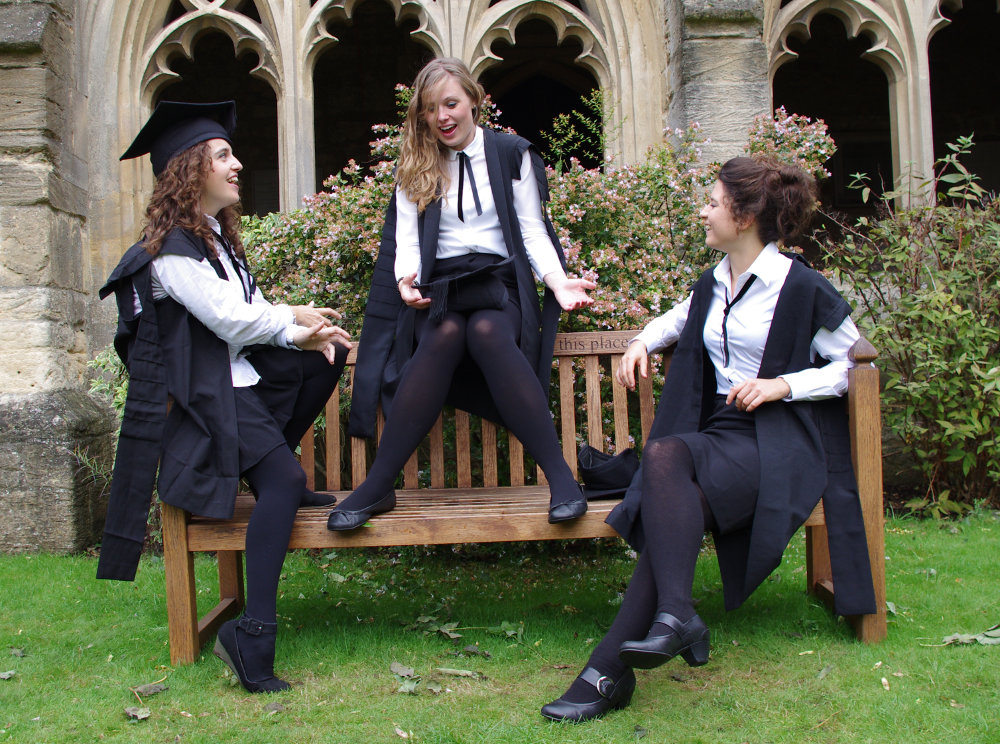
\includegraphics[width=0.9\textwidth]{subfusc2.jpg}
				\caption[]{Oxford natives in traditional costumes}
				\label{fig:subfusc}
        \end{minipage}%
        \quad
		\begin{minipage}{0.38\textwidth}
        	\centering
				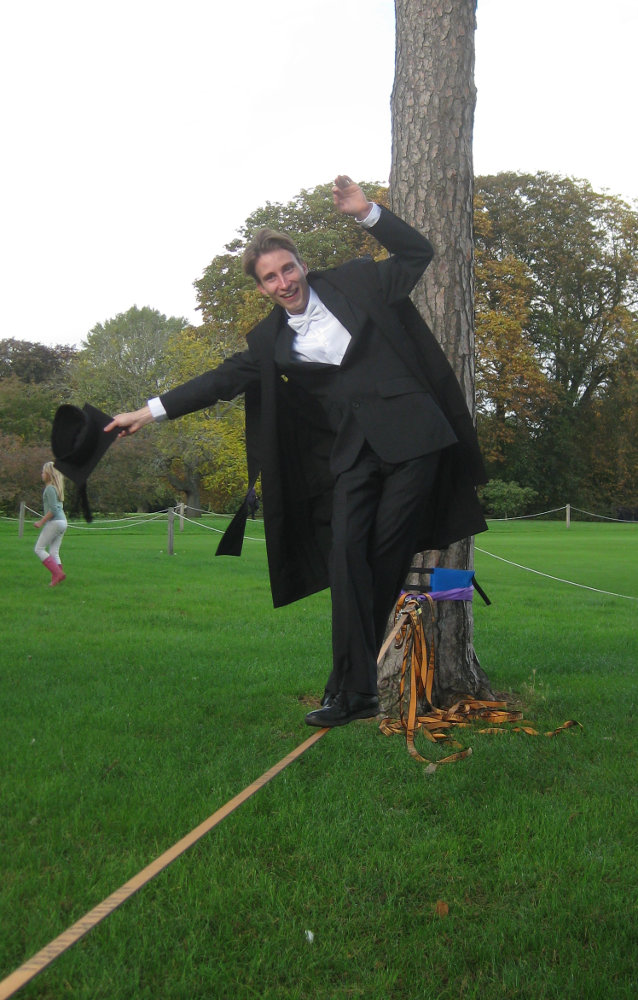
\includegraphics[width=0.9\textwidth]{subfusc.jpg}
				\caption[]{\emph{EVERYTHING} in Oxford is done in sub fusc and
				gown!}
				\label{fig:slack}
        \end{minipage}%
\end{figure}  
  
\section{Bicycles}
Some people cannot live without their bike in Oxford, whilst others get by fine
without one. A lot depends on your lifestyle, particularly the distance between
your accommodation and where you will be spending most of your time working
(department/lab/favourite library). Buying a new bike in Oxford can be expensive
but due to the high bike-to-person ratio there is a large second-hand market.
The \href{http://www.dailyinfo.co.uk/}{\urlformat{DailyInfo}} website is a good place to start looking (as are the usual websites such as Gumtree), and expect to pay more than \pounds50. Bike theft is
the most common crime committed against Oxford students, so a high-quality
D-lock is essential (\pounds15 for students
\url{https://www.admin.ox.ac.uk/ouss/cra/cyclesecurity/}).

\section{Welfare}
College provides a constellation of people attuned to all manner of welfare matters: there are the Cox and Salvesen Fellows, both experts in the ways of pastoral care; the Chaplain, who can advise on any issue, spiritual or otherwise; the porters, frequently indispensable in times of need; the Dean, the Assistant Dean, and the two Junior Deans; as well as our MCR welfare officer and trained peer supporters. See below for contact information.

\medskip

\begin{table}[!h]
\centering
\begin{tabular}{ >{\bfseries}l l}
\toprule
Welfare Contacts & Telephone and e-mail \\
\midrule
Main Porters' Lodge	&			(01865~2)79500 \\
Weston Porters' Lodge	&		(01865~2)81081 \\
Nightline (8\,pm-8\,am, 0th-9th week) &	(01865~2)70270 \\
Counselling Service & 			(01865~2)70300\\
					&			\href{mailto:reception@counserv.ox.ac.uk}{\urlformat{reception@counserv.ox.ac.uk}} \\
Student Advice Service &		\href{mailto:advice@ousu.org}{\urlformat{advice@ousu.org}} \\
Emergency				&		999\\
\bottomrule
\end{tabular}
\caption{Welfare Contacts}
\label{tab:welfcontact}
\end{table}

\begin{table}[!h]
\centering
\begin{tabular}{ >{\bfseries}l l}
\toprule
New College Welfare Team & Telephone and e-mail \\
\midrule
Erica Longfellow, Chaplain (3OB6)	& (01865~2)79451 \\
						& \href{mailto:erica.longfellow@new.ox.ac.uk}{\urlformat{erica.longfellow@new.ox.ac.uk}} \\
Tom Cutterham, Cox Fellow &			(01865~2)79514 \\
						& \href{mailto:tom.cutterham@new.ox.ac.uk}{\urlformat{tom.cutterham@new.ox.ac.uk}} \\
Ryan Hanley, Salvesen Fellow & 		(01865~2)79531 \\
						& \href{mailto:ryan.hanley@new.ox.ac.uk}{\urlformat{ryan.hanley@new.ox.ac.uk}} \\
Caroline Thomas, Domestic Bursar &	(01865~2)79560 \\
						& \href{mailto:caroline.thomas@new.ox.ac.uk}{\urlformat{caroline.thomas@new.ox.ac.uk}}\\ 
\bottomrule
\end{tabular}
\caption{New College Welfare Team}
\label{tab:welfcollege}
\end{table}

\begin{table}[!h]
\centering
\begin{tabular}{ >{\bfseries}l l}
\toprule
MCR Peer Supporters & e-mail \\
\midrule

Belinda Faust (Welfare Officer)	& \href{mailto:belinda.faust@new.ox.ac.uk}{\urlformat{belinda.faust@new.ox.ac.uk}} \\
Martin Hallmannsecker (LGBTQ+ officer) & \href{mailto:martin.hallmannsecker@new.ox.ac.uk}{\urlformat{martin.hallmannsecker@new.ox.ac.uk}} \\
Cristina Golomoz (Women's Officer)	& \href{mailto:cristina.golomoz@new.ox.ac.uk}{\urlformat{cristina.golomoz@new.ox.ac.uk}} \\
Erika Lam (Peer Supporter)	& \href{mailto:erika.lam@new.ox.ac.uk}{\urlformat{erika.lam@new.ox.ac.uk}} \\
Richard Millar (Peer Supporter)	& \href{mailto:richard.millar@new.ox.ac.uk}{\urlformat{richard.millar@new.ox.ac.uk}} \\
\bottomrule
\end{tabular}
\caption{Peer Supporters}
\label{tab:peersupp}
\end{table}

Please note that the phone numbers without brackets are from internal lines (e.g. using the phone in your room at Weston). From outside lines, including your own mobile, dial the area code 01865, then 2 and then the number. Please make an appointment in advance (preferably via email) to see the Cox or the Salvesen Fellow. In an emergency, however, contact the Porters' Lodge and they will get in touch with a member of the welfare team for you straight away

\section{LGBTQ+ students}
There is a lot going on at Oxford for lesbian, gay, bisexual, transexual and
intersex students. The College may date from 1379, and the University from about
200 years before that, but you'll find that attitudes have moved on a long way
since then. There are LGBTQ students in the New College MCR and all across the
town and University, so there will be plenty of friendly faces to show you the
sights and give you the insiders' tips on the best places to go out.
Alternatively, get in touch with the lovely Hamish
(\href{mailto:martin.hallmannsecker@new.ox.ac.uk}{\urlformat{martin.hallmannsecker@new.ox.ac.uk}}), your very own LGBTQ+ rep on the MCR committee, who keeps you updated with all the weekly events and is always approachable in case you need someone to talk to. OU LGBTQ+ Society (\url{http:// oulgbtsoc.com}) has heaps of info on their website, and is a great group to join with lots of fun social events. Keep your eyes out for the OUSU LGBT handbook, and OUSU also have a Queer Rights group if you are interested in the more activist side of things. More information on freshers' events outside college will be available in freshers' fortnight.

\section{Terms}
Oxford has three terms: Michaelmas from October to December; Hilary from January
to March; Trinity from April to June. Terms formally last eight weeks: weeks
'start' on Sunday and are numbered from one through to eight. Thus, within
Oxford, you tend to describe dates using this system: so, for example, you might
say, \emph{my exam is on Tuesday of 7th week}. The week before first is called
0th week and the one before that minus 1st week etc. The gaps between terms are the \emph{Christmas}, \emph{Easter} and \emph{Long} vacations.
\medskip

Undergraduate teaching takes place during weeks of full term. For those doing taught courses, teaching will be focused during term but you may well have to do assignments out of term: so check this before you book a six week holiday in the Easter vacation! For research students terms are less relevant, and what time you get away is largely up to you and your supervisor.

\section{Transportation}

The public transport system in and around Oxford relies mainly on the
\href{http://www.oxfordbus.co.uk/}{\urlformat{Oxford Bus Company}} buses, the
single fare in the centre region is \pounds1, to be paid to the driver (they
prefer exact change).

The main connections to London are run by the
\href{http://www.oxfordtube.com/}{\urlformat{Oxford Tube}}, a bus line from
Oxford's central bus station at Gloucester Green to London Victoria, and
\href{https://www.firstgreatwestern.co.uk/}{\urlformat{First Great Western}},
the train carrier connecting Oxford to London Paddington. Both offer various fares depending on booking date,
return date, number of tickets bought, etc. The cheapest fare for both of them
is \pounds10-12 for a return ticket, but the availability conditions
vary.

There is now also a new train connection between Oxford and London Marleybone run by \href{https://www.chilternrailways.co.uk/}{\urlformat{Chiltern Railways}}. 

Luton and Standsted airports can be reached by bus via
\href{http://www.nationalexpress.com/}{\urlformat{National Express}}, Heathrow
and Gatwick via the \href{http://airline.oxfordbus.co.uk/}{\urlformat{Airline}},
a bus operated by the Oxford Bus Company.
Tickets for all of them can be bought via the
\href{http://www.nationalexpress.com/}{\urlformat{National Express page}}, the
Airline tickets also via the \href{https://airlinebooking.oxfordbus.co.uk/}{\urlformat{Airline page}}.
Fares vary depending on time of day, advance booking, return dates and other
more mysterious criteria. A single trip to Luton costs up to \pounds18, to
Heathrow up to \pounds25, to Stansted up to \pounds27 and to Gatwick up to \pounds30,
return and off peak tickets are often cheaper.
In many cases creative routes can lower the costs (e.g. taking the bus from
Gatwick to Victoria, followed by the Oxford Tube to Oxford comes to \pounds21),
as can
\href{http://www.nationalexpress.com/waystosave/young-persons-coachcard.aspx}
{\urlformat{Coachcards}}
and \href{http://www.railcard.co.uk/}{\urlformat{Railcards}}, which allow you to
save a fixed percentage of the fare for many routes. Their usefulness depends heavily on your travel style, but they may be worth a look.
